\section{IPOL web interface}

current version is 3.0.

\subsection{Introduction}
The IPOL Demo Web Interface has been developed with HTML5, CSS3, and JQuery. 
It allows the users to execute the IPOL algorithms with an ergonomic interface. The users can use their own data or the examples offered by each of the demos. We shall describe the modules of which the web interface is made, its flow diagram, how the asynchronous calls work, and the data types accepted.

\section{Modules}
The Javascript application is made of the following modules:

\begin{itemize}
	\item Inputs
	\item Upload
	\item Editor
	\item Parameters
	\item Run
	\item Results
	\item Helpers 
\end{itemize}

Each of these items is described in the following sections.

\subsection{Inputs}
This module manages the list of blobs used as examples in the demo and renders them on the web page. This module is the first which is loaded and it communicates with the DemoInfo and Blobs modules, see Fig. \ref{fig:server_interaction}.

This input module allows the user to choose one or many blobs in the demo. These blobs are be for example images, videos, or audio blobs. It displays a line of blobs or sets of blobs to choose from.


\subsection{Upload}
If the users want to use their own blobs for the demo this module lets you upload them. Every demo has predefined 
upload slots each with their own characteristics like maximum file size and maximum image size. The user is able to upload the 
minimum required number of uploads. This module listen for events in every upload slot and get the file information in order to 
upload them when the run button is pressed.


\subsection{Editor}
This module loads after the user selects a set of blobs to run the demo with or when the users upload their blobs. It loads a view of
the chosen blobs where there is a zoom and crop functions when the sets have one blob per set. When the sets have more than 
one blob per set, the user will have the possibility to compare them with the corresponding 'Compare button', but not a crop 
an area.

\subsection{Parameters}
This module renders the parameters of the demo described in the DDL after the user chooses blobs to use with the demo. 
Parameters have as many types DDL specifies, so the interface renders each type accordingly.

\subsection{Run}
This module will send all the blobs and requirements needed to run the demo on the servers and will send this information to 
the core module. The answer will be either a success message with enough information to render the results or an error message 
that will show an approximation of what failed during execution.

\subsection{Results}
This module renders the results returned by the core letting the user compare the input and results, based on the ddl results section. 


\subsection{Helpers}
This module act as an interface for common utility methods like read and write to sessionStorage, make HTTP requests and 
read the origin of the chosen blobs for the demo, this could be blobset, meaning blobs are chosen from the ones offered by the 
demo, and upload, meaning the user has uploaded his own blobs.

\begin{figure}[ht]
	\centering
	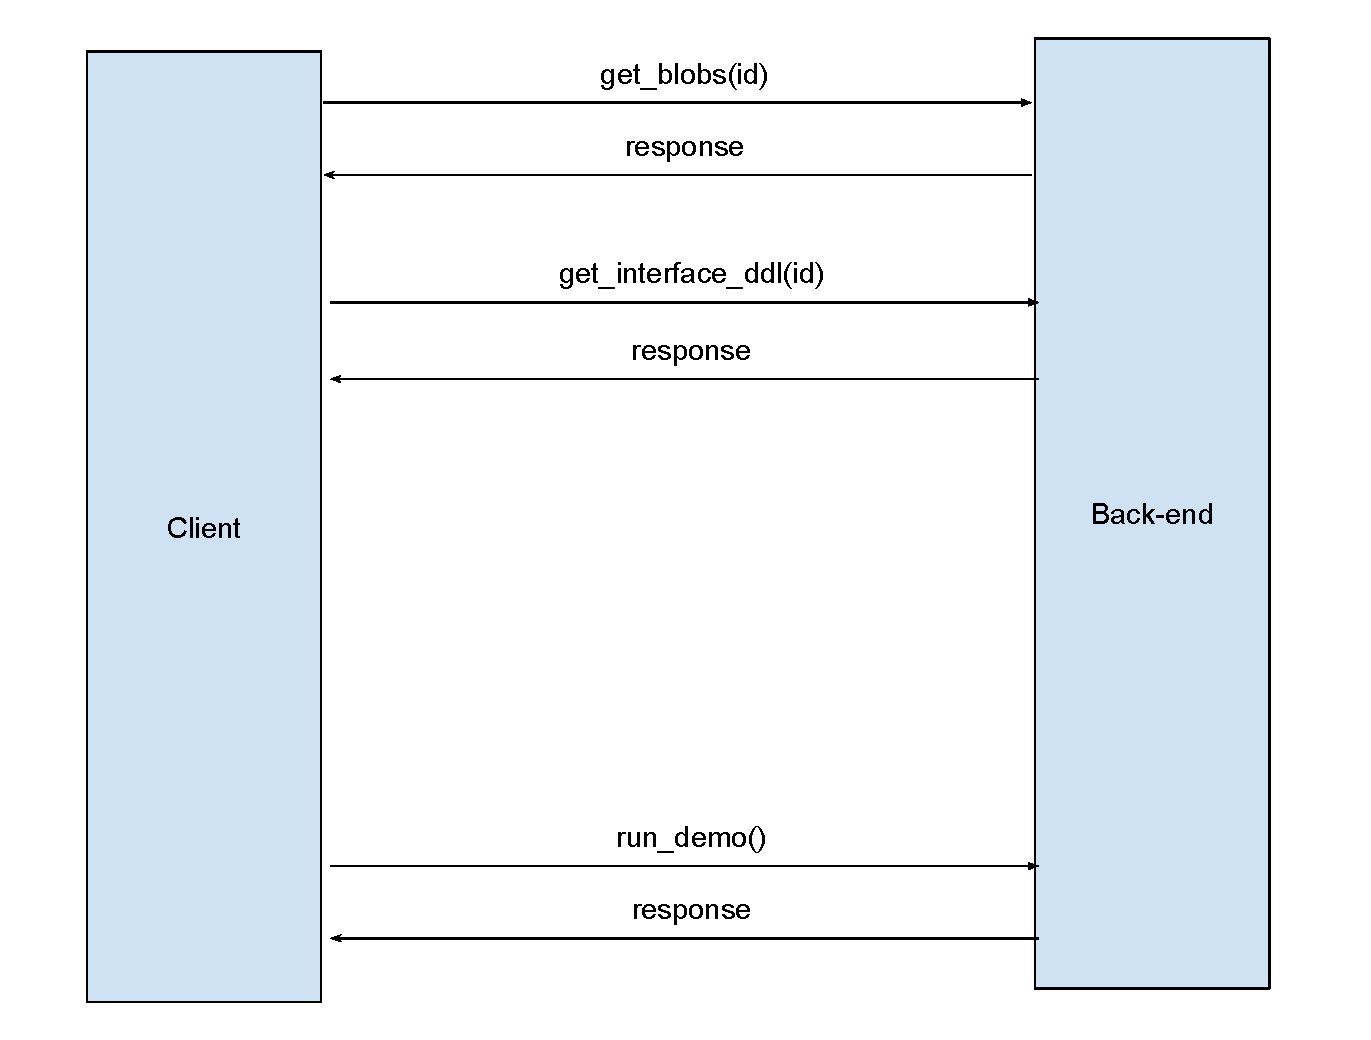
\includegraphics[width=\textwidth]{images/client_server_interaction}
	\caption{Client-server interation} 
	\label{fig:server_interaction}
\end{figure}

%--------------------------------------------------------------------------------

\section{Flow diagram}
When the application is loaded, the input module will locate the demo according to its ID. This ID is a get parameter from the URL.
Once the demo has this ID parameter, the main file, demo.js will load the different html files into the DOM. They have been divided 
into several files to improve maintainability and coupling.

After this process is done, the app will continue rendering the main section to the DOM, containing in this case the blobs viewer and 
the blob upload dialog. The information regarding the DDL and the blobs specification will be saved in sessionStorage once it has been retrieved by the asynchronous calls for easy access.

\begin{figure}[h]
	\centering
	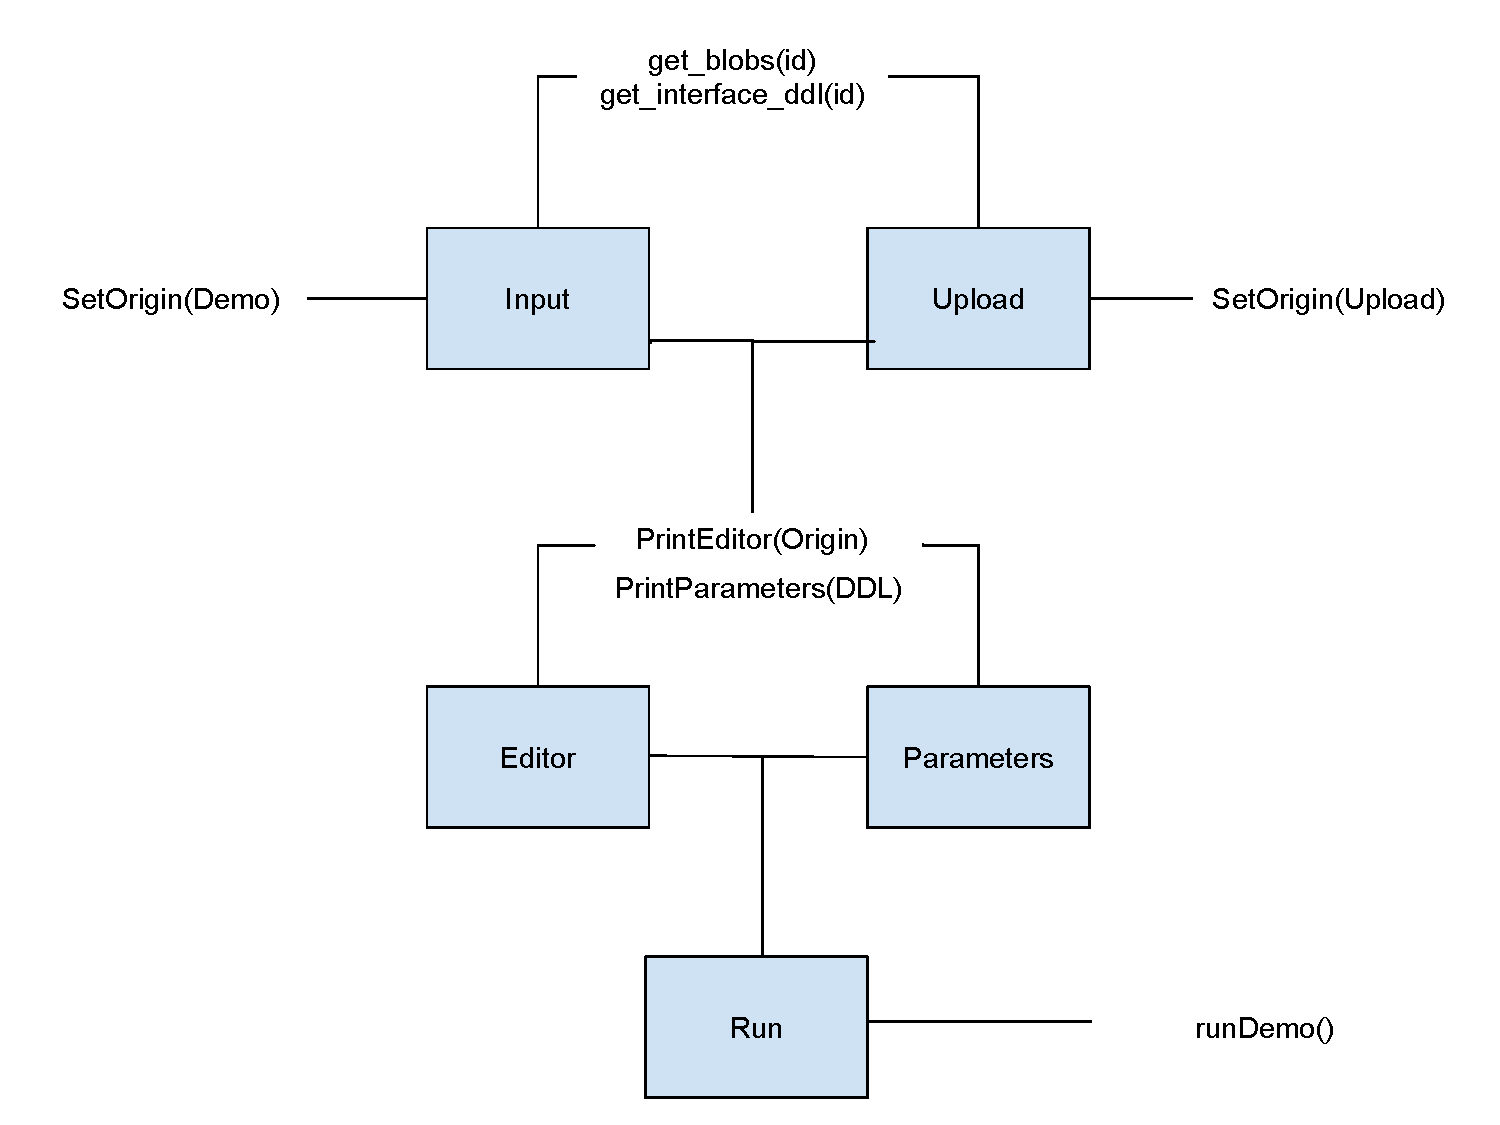
\includegraphics[width=\textwidth]{images/flow}
	\caption{Flow diagram} 
	\label{fig:flow_diagram}
\end{figure} 


As shown in figure  \ref{fig:flow_diagram}, either input or upload modules will pass 
information to the following modules. Each will set a variable in sessionStorage that will indicate if the user has chosen to 
upload blobs for the demo or a default blob from the list. If this variable is not set, it means the demo has no inputs defined 
in the DDL.

After the user chooses a blob, the editor and parameter modules will load independently and wait for changes. The Editor control 
will allow to either zoom, crop, and compare blobs if it is possible, as well as do inpainting operations when the demo requires it. 
The parameters will be modifiable according to the DDL specification values and will be stored in a variable in order to achieve 
parameter visibility dependence and to send this data when the run button is pressed.

After the user hits the run button an HTTP post will be executed to run the demo and send the necessary information and wait for 
a response. When the response is obtained it will either print the results interface or the error message.

%--------------------------------------------------------------------------------

\subsection{Sharing results}
Every time you run a demo, the URL will change to include the run key. This key allows the user to share the relatively short URL 
with anyone. Sharing will allow other users to see the parameters, results and inputs including crop information exactly just as the 
demo was executed by the original user. 

\subsection{Private mode}
This functionality allows the user to do a private execution of the demo. This makes the system not to record anything in the archives when running 
a demo. So nobody will see the execution results unless you share the URL with the execution key to someone. To activate private 
mode there is a checkbox in the lower part of the upload dialog.

\subsection{External modules}

The IPOL demo Web interface uses external libraries for extra functionalities.
Currently it uses:

\begin{itemize}
\item Cropper.js: Cropper.js it is a simple image cropping JQuery plugin. It is used in the editor panel with the image blobs.
\end{itemize}

%--------------------------------------------------------------------------------

\subsection{Async calls}
The IPOL demo Web interface uses asynchronous calls to get the necessary information from the IPOL server.

The current version uses asynchronous calls for:
\begin{itemize}
\item Get the demo DDL: Used to show the inputs description and the upload modal in the Inputs panel, also uses this information to show the parameters.
\item Get blobs: Used to show the blobs in the inputs panel.
\item Run demo: It will send all parameters needed to run the demo enclosed in the runData variable and will respond with either the results of 
the demo or an error response.
\end{itemize}

%--------------------------------------------------------------------------------

\subsection{Data types}
The IPOL platform supports images, audio and video files to use in demos. The new web interface 
allows to choose a set with any combination of images, audio and video. Depending on the data types and sets length options will vary. 
If a set contains multiple images, the user will be able to compare and make zoom using any image on the set. If the user chooses a set with only 
one image blob, options will depend on DDL limitations and will include zoom and crop features, as well as inprinting editing.

\section{Implementation of Features}
This section describes how particular features on the web interface are implemented.

%
\subsection{Execution recovery}
It is common that a researcher get an interesting result after executing a demo with some particular input and parameters and want to share with a colleague. The first intuition is to simple copy the URL shown in the browser and ask the other persons to paste it in their browsers, to get the same page. Note that this is different from browsing the archive or to recover an archived experiment.

The IPOL webpage is AJAX dynamic and therefore this need that the web interface and the backend do dome extra work. The idea is to save the \emph{state} of the page after the execution, including the origin of the blobs used (uploaded original content or examples from the demo), the crop, parameters, and the results displayed. In general, any data needed to recover the same page state.

After the execution of the demo the Core module saves the run request and the corresponding response into a {\tt execution.json} text file after the web interface requests the {\tt save\_execution} service. This file is saved at the temporal execution folder.
%
When the web interface needs to recover the state of the page it invokes the {\tt load\_execution} service of the Core along with the demo ID and the execution key. The Core reads the text file and sends back to the web interface all the information needed to put the demo page in the apropriate state.

The interaction diagram is shown in Fig. \ref{fig:execution_flow}.

\begin{figure}[h]
	\centering
	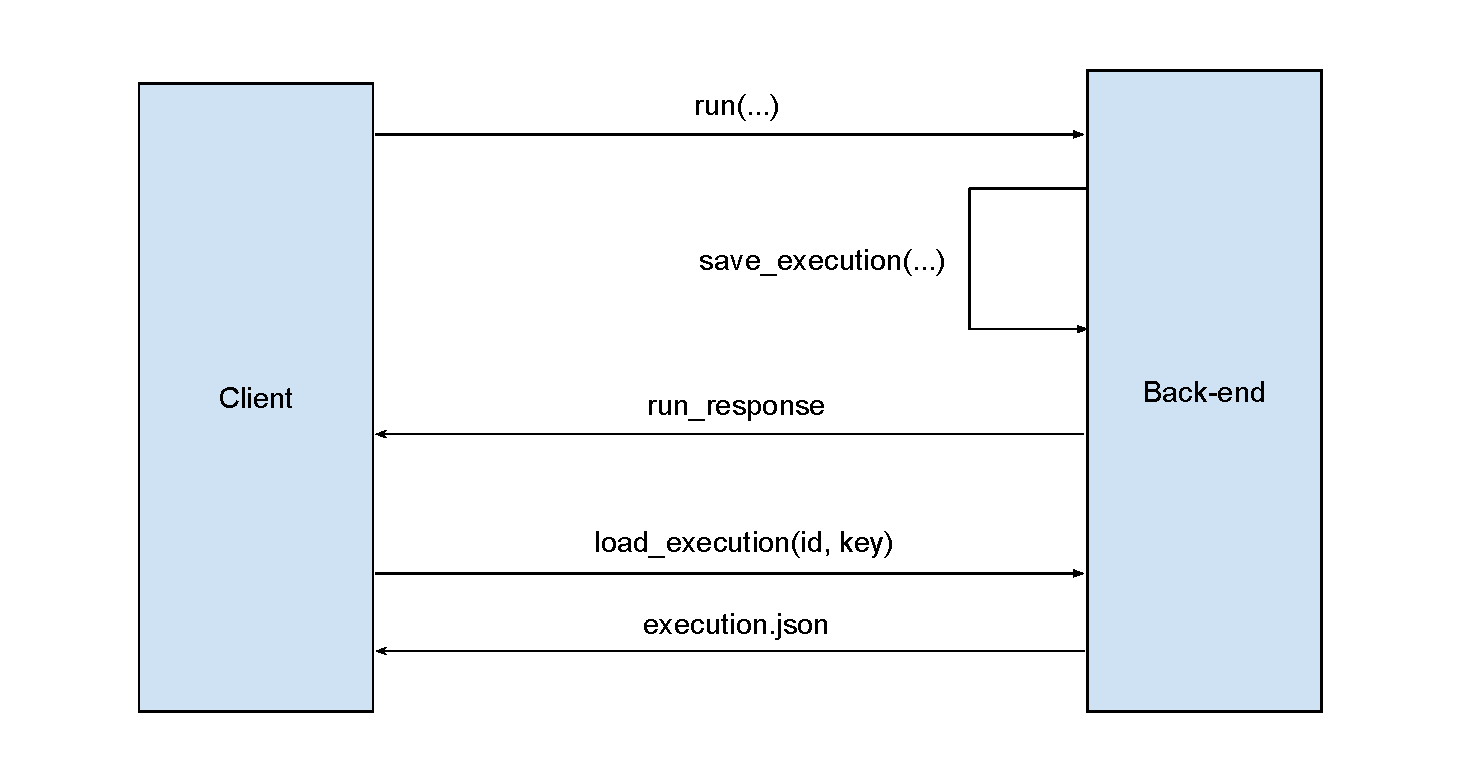
\includegraphics[width=\textwidth]{images/execution_flow}
	\caption{Execution flow diagram for the functionality of saving/recovering the state of the demo page.} 
	\label{fig:execution_flow}
\end{figure}
